\chapter{Лабораторная работа №1\\Введение в Verilog HDL} 
\section{Возникновение языков описания цифровой аппаратуры}

\par{Цифровые устройства — это устройства, предназначенные для приёма и обработки цифровых сигналов. Цифровыми называются сигналы, которые можно рассматривать в виде набора дискретных уровней. В цифровых сигналах информация кодируется в виде конкретного уровня напряжения. Как правило выделяется два уровня — логический «0» и логическая «1».}

\par{Цифровые устройства стремительно развиваются с момента изобретения электронной лампы, а затем транзистора. Со временем цифровые устройства стали компактнее, уменьшилось их энергопотребление, возросла вычислительная мощность. Так же разительно возросла сложность их структуры.}

\par{Графические схемы, которые применялись для проектирования цифровых устройств на ранних этапах развития, уже не могли эффективно использоваться. Потребовался новый инструмент разработки, и таким инструментом стали языки описания аппаратной части цифровых устройств (\eng{Hardware Description Languages, HDL}), которые описывали цифровые структуры формализованным языком, чем-то похожим на язык программирования.}

\par{Совершенно новый подход к описанию цифровых схем, реализованный в языках \eng{HDL}, заключается в том, что с их помощью можно описывать не только структуру, но и поведение цифрового устройства. Окончательная структура цифрового устройства получается путём обработки таких смешанных описаний специальной программой — синтезатором.}

\par{Такой подход существенно изменил процесс разработки цифровых устройств, превратив громоздкие, тяжело читаемые схемы в относительно простые и доступные описания поведения.}

\par{В данном курсе мы рассмотрим язык описания цифровой аппаратуры \eng{Verilog HDL} — один из наиболее распространённых на текущий момент. И начнём мы с разработки наиболее простых цифровых устройств — логических вентилей.}

\section{\eng{HDL} описания логических вентилей}

\par{Логические вентили реализуют функции алгебры логики: И, ИЛИ, Исключающее ИЛИ, НЕ. Напомним их таблицы истинности:}

\begin{table}[!htbp]
  \parbox{.45\linewidth}{
    \centering
  \begin{tabular}{c|c|c}
    $a$&$b$&$a \cdot b$\\
    \hline
    $0$ & $0$ & $0$ \\
    $0$ & $1$ & $0$ \\
    $1$ & $0$ & $0$ \\
    $1$ & $1$ & $1$ \\
  \end{tabular}
  \caption{И}
} \hfill
  \parbox{.45\linewidth}{
    \centering
  \begin{tabular}{c|c|c}

    $a$&$b$&$a | b$\\
    \hline
    $0$ & $0$ & $0$ \\
    $0$ & $1$ & $1$ \\
    $1$ & $0$ & $1$ \\
    $1$ & $1$ & $1$ \\

  \end{tabular}
  \caption{ИЛИ}
}\hfill
  \parbox{.45\linewidth}{
    \centering
  \begin{tabular}{c|c|c}
    $a$&$b$&$a \xor b$\\
    \hline
    $0$ & $0$ & $0$ \\
    $0$ & $1$ & $1$ \\
    $1$ & $0$ & $1$ \\
    $1$ & $1$ & $0$ \\
  \end{tabular}
  \caption{Исключающее ИЛИ}
}\hfill
  \parbox{.45\linewidth}{
    \centering
  \begin{tabular}{c|c}
    $a$&$\bar{a}$\\
    \hline
    $0$ & $1$\\
    $1$ & $0$\\
  \end{tabular}
  \caption{НЕ}
}
\end{table}

\par{Начнём знакомиться с \eng{Verilog HDL} с описания логического вентиля \quotes{И}. Ниже приведен код, описывающий вентиль с точки зрения его структуры:}

\noindent
\begin{minipage}{\linewidth}
 \lstinputlisting[caption={Модуль, описывающий вентиль \quotes{И}}]{./code_examples/lab_1/and_gate.v}
\end{minipage}

\par{Описанный выше модуль можно представить как некоторый \quotes{ящик}, в который входит 2 провода с названиями \emph{\qeng{a}} и \emph{\qeng{b}} и из которого выходит один провод с названием \emph{\qeng{result}}. Внутри этого блока результат выполнения операции \quotes{И} (в синтаксисе Verilog записывается как \quotes{\&}) над входами соединяют с выходом.}
\par{Схематично изобразим этот модуль:}

\begin{figure}[H]
  \centering
  \def\svgwidth{\columnwidth}
  \includesvg{images/lab_1/and_gate}
  \caption{Структура модуля \qeng{and\_gate}}
\end{figure}

\par{Аналогично опишем все оставшиеся вентили:}

\noindent
\begin{minipage}{\linewidth}
  \lstinputlisting[caption={Модуль, описывающий вентиль \quotes{ИЛИ}}]{./code_examples/lab_1/or_gate.v}
\end{minipage}

\noindent
\begin{minipage}{\linewidth}
  \lstinputlisting[caption={Модуль, описывающий вентиль \mbox{\quotes{Исключающее ИЛИ}}}]{./code_examples/lab_1/xor_gate.v}
\end{minipage}

\noindent
\begin{minipage}{\linewidth}
  \lstinputlisting[caption={Модуль, описывающий вентиль \quotes{НЕ}}]{./code_examples/lab_1/not_gate.v}
\end{minipage}

\par{В проектировании цифровых устройств логические вентили наиболее часто используются для формулировки и проверки сложных условий, например:}

\lstinputlisting[caption={Пример использования логических вентилей}]{./code_examples/lab_1/logic_gatex_example.v}

\par{Условие будет выполняться либо когда \emph{не} выполнено условие \emph{\qeng{c}}, либо когда одновременно выполняются условия \emph{\qeng{a}} и \emph{\qeng{b}}. \emph{Здесь и далее под условием понимается логический сигнал, отражающий его истинность.}}
\par{В качестве входов, выходов и внутренних соединений в блоках могут использоваться шины — группы проводов. Ниже приведен пример работы с шинами:}

\lstinputlisting[caption={Модуль, описывающий побитовое \quotes{ИЛИ} \mbox{между двумя шинами}},float,floatplacement=H]{./code_examples/lab_1/bus_or.v}

\par{Это описание описывает побитовое \quotes{ИЛИ} между двумя шинами по 8 бит. То есть описываются восемь логических вентилей \quotes{ИЛИ}, каждый из которых имеет на входе соответствующие разряды из шины \emph{\qeng{x}} и шины \emph{\qeng{y}}.}

\par{При использовании шин можно в описании использовать конкретные биты шины и группы битов. Для этого используют квадратные скобки после имени шины:}

\lstinputlisting[caption={Модуль, демонстрирующий \mbox{битовую адресацию шин}}, ]{./code_examples/lab_1/bitwise_ops.v}

\par{Такому описанию соответствует следующая структурная схема, приведённая на Рис. \ref{fig:bitwiseops}}

\begin{figure}[H]
  \centering
  \def\svgwidth{\columnwidth}
  \includesvg{images/lab_1/bitwise_ops}
  \caption{Структура модуля \qeng{bitwise\_ops}}
  \label{fig:bitwiseops}
\end{figure}

\par{Впрочем, реализация ФАЛ (функций алгебры логики) с помощью логических вентилей не всегда представляется удобной. Допустим нам нужно описать таблично-заданную ФАЛ. Тогда для описания этой функции при помощи логических вентилей нам придётся сначала минимизировать её и только после этого, получив логическое выражение (которое, несмотря на свою минимальность, не обязательно является коротким), сформулировать его с помощью языка \eng{Verilog HDL}. Как видно, ошибку легко допустить на любом из этих этапов.}

\par{Одно из главных достоинств \eng{Verilog HDL} — это возможность описывать поведение цифровых устройств вместо описания их структуры.}

\par{Программа-синтезатор анализирует синтаксические конструкции поведенческого описания цифрового устройства на \eng{Verilog HDL}, проводит оптимизацию и, в итоге, вырабатывает структуру, реализующую цифровое устройство, которое соответствует заданному поведению.}

\par{Используя эту возможность, опишем таблично-заданную ФАЛ на \eng{Verilog HDL}:}

\lstinputlisting[caption={Пример описания таблично-заданной ФАЛ на \eng{Verilog HDL}}, ]{./code_examples/lab_1/function_example.v}

\par{Описание, приведённое выше, определяет $y$, как таблично-заданную функцию, которая равна нулю на наборах 0, 2, 5, 6, 7 и единице на всех остальных наборах.}

\par{Остановимся подробнее на новых синтаксических конструкциях:}
\par{Описание нашего модуля начинается с создания трёхбитной шины \qeng{x\_bus} на строке 7.}
\par{После создания шины \qeng{x\_bus} она подключается к объединению проводов \qeng{x2}, \qeng{x1} и \qeng{x0} с помощью оператора \eng{assign} как показано на Рис. \ref{fig:assign}.}

\begin{figure}[H]
  \centering
  \def\svgwidth{\columnwidth}
  \includesvg{images/lab_1/assign}
  \caption{Действие оператора \kword{assign}}
  \label{fig:assign}
\end{figure}

\par{Затем начинается функциональный блок \kword{always}, на котором мы остановимся подробнее.}
\par{\eng{Verilog HDL} описывает цифровую аппаратуру, которая существует вся одновременно, но инструменты анализа и синтеза описаний являются программами и выполняются последовательно на компьютере. Так возникла необходимость последовательной программе «рассказать» про то, какие события приводят к срабатыванию тех или иных участков кода. Сами эти участки назвали процессами. Процессы обозначаются ключевым словом \kword{always}.}

\par{В скобках после символа @ указывается так называемый \emph{список чувствительности процесса}, т.е. те сигналы, изменение которых должно приводить к пересчёту результатов выполнения процесса.}


\par{Например, результат ФАЛ надо будет пересчитывать каждый раз, когда изменился входной вектор (любой бит входного вектора, т.е. любая переменная ФАЛ). Эти процессы можно назвать блоками или частями будущего цифрового устройтсва.}


\par{Новое ключевое слово \kword{reg} здесь необходимо потому, что в выходной вектор происходит запись, а запись в языке \eng{Verilog HDL} разрешена только в «регистры» — специальные «переменные», предусмотренные в языке. Данная концепция и ключевое слово reg будет рассмотрено гораздо подробнее в следующей лабораторной работе.}

\par{Оператор \kword{<=} называется оператором \emph{неблокирующего присваивания}. В результате выполнения этого оператора то, что стоит справа от него, «помещается» («кладется», «перекладывается») в регистр, который записан слева от него. Операции неблокирующего присваивания происходят одновременно по всему процессу.}

\par{Оператор \kword{case} описывает выбор действия в зависимости от анализируемого значения. В нашем случае анализируется значение шины \qeng{x\_bus}. Ключевое слово \kword{default} используется для обозначения всех остальных (не перечисленных) вариантов значений.}

\par{Константы и значения в языке \eng{Verilog HDL} описываются следующим образом: сначала указывается количество бит, затем после апострофа с помощью буквы указывается формат и, сразу за ним, записывается значение числа в этом формате.}

\par{Возможные форматы:
  \begin{itemize}[noitemsep,topsep=0pt, after=\vspace{2pt}]
    \item b – бинарный, двоичный;
    \item o - восьмеричный;
    \item h – шестнадцатеричный;
    \item d – десятичный.
  \end{itemize}}

\par{Немного расширив это описание, легко можно определить не одну, а сразу несколько ФАЛ одновременно. Для упрощения записи сразу объединим во входную шину все переменные. В выходную шину объединим значения функций:}

\lstinputlisting[caption={Описание дешифратора на языке \eng{Verilog}}, ]{./code_examples/lab_1/decoder.v}

\par{Теперь нам удалось компактно записать четыре функции, каждая от трёх переменных:
\begin{itemize}[noitemsep,topsep=2pt,label={}]
  \item $y_0=f(x_2,x_1,x_0);$
  \item $y_1=f(x_2,x_1,x_0);$
  \item $y_2=f(x_2,x_1,x_0);$
  \item $y_3=f(x_2,x_1,x_0).$
\end{itemize}}

\par{Но, если мы посмотрим на только что описанную конструкцию под другим углом, мы увидим, что это описание можно трактовать следующим образом: \quotes{поставить каждому возможному входному вектору $x$ в соответствие заранее определенный выходной вектор $y$}. Такое цифровое устройство называют \emph{дешифратором}.}

\par{На Рис. \ref{fig:decoder} показано принятое в цифровой схемотехнике обозначение дешифратора.}

\begin{figure}[H]
  \centering
  \def\svgwidth{\columnwidth}
  \includesvg{images/lab_1/decoder}
  \caption{Графическое обозначение дешифратора}
  \label{fig:decoder}
\end{figure}

\par{Заметим, что длины векторов не обязательно должны совпадать, а единственным условием является полное покрытие всех возможных входных векторов, что, например, может достигаться использованием условия \kword{default} в операторе \kword{case}.}

\par{Дешифраторы активно применяются при разработке цифровых устройств. В большинстве цифровых устройств в явном или неявном виде можно встретить дешифратор.}

\par{Рассмотрим еще один интересный набор ФАЛ:}

\lstinputlisting[caption={Описание мультиплексора на языке \eng{Verilog}}, ]{./code_examples/lab_1/multiplexer.v}

\par{Что можно сказать об этом описании? Выходной вектор $y$ — это результат работы трёх ФАЛ, каждая из которых является функцией 6 переменных. Так, $y_0 = f(a_0, b_0, c_0, d_0, s_1, s_0)$.}

\par{Анализируя оператор \kword{case}, можно увидеть, что главную роль в вычислении значения ФАЛ играет вектор $s$, в результате проверки которого выходу ФАЛ присваивается значение \quotes{выбранной} переменной.}

\par{Получившееся устройство называется \emph{мультиплексор}}.

\par{Мультиплексор работает подобно коммутирующему ключу, замыкающему выход с выбранным входом. Для выбора входа мультиплексору нужен сигнал управления. }

\par{Графическое изображение мультиплексора приведено на Рис. \ref{fig:mux}}

\begin{figure}[H]
  \centering
  \def\svgwidth{\columnwidth}
  \includesvg{images/lab_1/mux}
  \caption{Графическое обозначение мультиплексора}
  \label{fig:mux}
\end{figure}

\par{Особенно хочется отметить, что на самом деле никакой \quotes{проверки} сигнала управления не существует и уж тем более не существует \quotes{коммутации}, ведь мультиплексор — это таблично-заданная ФАЛ. Результат выполнения этой ФАЛ выглядит так, как будто происходит \quotes{подключение} \quotes{выбранной} входной шины к выходной.}

\par{Приведём для наглядности таблицу, задающую ФАЛ для одного бита выходного вектора (число ФАЛ в мультиплексоре и, следовательно, число таблиц, равняется числу бит в выходном векторе). Для краткости выпишем таблицу наборами строк вида: $f(s_1, s_0, a_0, b_0, c_0, d_0) = y_0$ в четыре столбца.}

\par{Обратите внимание, что в качестве старших двух бит входного вектора для удобства записи и анализа мы выбрали переменные \quotes{управляющего} сигнала, а выделение показывает какая переменная \quotes{поступает} на выход функции $f$:}

\begin{longtable}{ c c c c}

  $f(00\bm{0}000) = 0$ & 
  $f(010\bm{0}00) = 0$ & 
  $f(1000\bm{0}0) = 0$ & 
  $f(11000\bm{0}) = 0$ \\ 

  $f(00\bm{0}001) = 0$ & 
  $f(010\bm{0}01) = 0$ & 
  $f(1000\bm{0}1) = 0$ & 
  $f(11000\bm{1}) = 1$ \\ 

  $f(00\bm{0}010) = 0$ & 
  $f(010\bm{0}10) = 0$ & 
  $f(1000\bm{1}0) = 1$ & 
  $f(11001\bm{0}) = 0$ \\ 

  $f(00\bm{0}011) = 0$ & 
  $f(010\bm{0}11) = 0$ & 
  $f(1000\bm{1}1) = 1$ & 
  $f(11001\bm{1}) = 1$ \\ 

  $f(00\bm{0}100) = 0$ & 
  $f(010\bm{1}00) = 1$ & 
  $f(1001\bm{0}0) = 0$ & 
  $f(11010\bm{0}) = 0$ \\ 

  $f(00\bm{0}101) = 0$ & 
  $f(010\bm{1}01) = 1$ & 
  $f(1001\bm{0}1) = 0$ & 
  $f(11010\bm{1}) = 1$ \\ 

  $f(00\bm{0}110) = 0$ & 
  $f(010\bm{1}10) = 1$ & 
  $f(1001\bm{1}0) = 1$ & 
  $f(11011\bm{0}) = 0$ \\ 

  $f(00\bm{0}111) = 0$ & 
  $f(010\bm{1}11) = 1$ & 
  $f(1001\bm{1}1) = 1$ & 
  $f(11011\bm{1}) = 1$ \\ 

  $f(00\bm{1}000) = 1$ & 
  $f(011\bm{0}00) = 0$ & 
  $f(1010\bm{0}0) = 0$ & 
  $f(11100\bm{0}) = 0$ \\ 

  $f(00\bm{1}001) = 1$ & 
  $f(011\bm{0}01) = 0$ & 
  $f(1010\bm{0}1) = 0$ & 
  $f(11100\bm{1}) = 1$ \\ 

  $f(00\bm{1}010) = 1$ & 
  $f(011\bm{0}10) = 0$ & 
  $f(1010\bm{1}0) = 1$ & 
  $f(11101\bm{0}) = 0$ \\ 

  $f(00\bm{1}011) = 1$ & 
  $f(011\bm{0}11) = 0$ & 
  $f(1010\bm{1}1) = 1$ & 
  $f(11101\bm{1}) = 1$ \\ 

  $f(00\bm{1}100) = 1$ & 
  $f(011\bm{1}00) = 1$ & 
  $f(1011\bm{0}0) = 0$ & 
  $f(11110\bm{0}) = 0$ \\ 

  $f(00\bm{1}101) = 1$ & 
  $f(011\bm{1}01) = 1$ & 
  $f(1011\bm{0}1) = 0$ & 
  $f(11110\bm{1}) = 1$ \\ 

  $f(00\bm{1}110) = 1$ & 
  $f(011\bm{1}10) = 1$ & 
  $f(1011\bm{1}0) = 1$ & 
  $f(11111\bm{0}) = 0$ \\ 

  $f(00\bm{1}111) = 1$ & 
  $f(011\bm{1}11) = 1$ & 
  $f(1011\bm{1}1) = 1$ & 
  $f(11111\bm{1}) = 1$ \\ 
\end{longtable}

\section{Задание лабораторной работы}

Общая структурная схема проекта выполненной лабораторной работы показана на изображении ниже.

\begin{figure}[H]
  \centering
  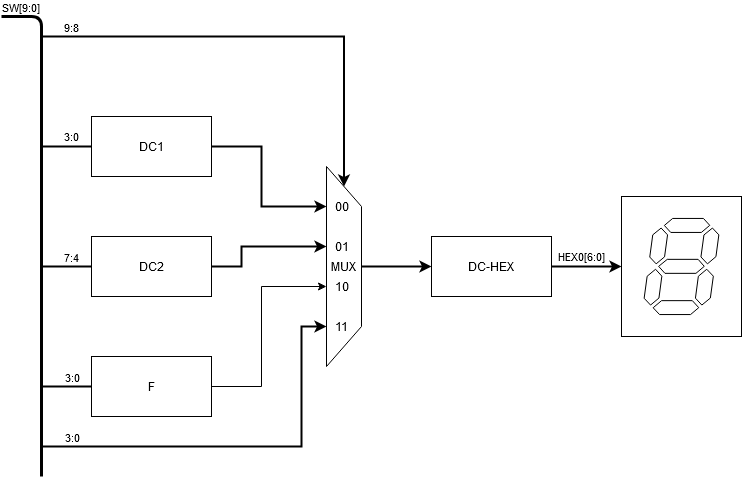
\includegraphics [width=1\textwidth] {images/lab_1/lab1_sch.png}
  \caption{Общая структурная схема проекта выполненной лабораторной работы.}
  %\label{lab1:pic1}
\end{figure}


\par{Описать на языке Verilog цифровое устройство, функционирующее согласно следующим принципам:}
\begin{enumerate}
  \item Ввод информации происходит с переключателей SW[9:0];
  \item SW[3:0] должны обрабатываться дешифратором «DC1», согласно индивидуальному заданию;
  \item SW[7:4] должны обрабатываться дешифратором «DC2», согласно индивидуальному заданию;
  \item Функция алгебры логики «F» должна принимать на вход сигналы SW[3:0].

  \item Реализовать дешифратор «DC-DEC», преобразующий число, представленное в двоичном коде в цифру, отображаемую на семисегментном индикаторе. Руководствоваться при этом нужно следующими соображениями:
    \begin{itemize}
      \item Семисегментный индикатор подключается к шине HEX0[6:0]
      \item Диоды на семисегментном индикаторе загораются при подаче на них низкого напряжения (0 - горит, 1 - не горит)
      \item Соответствие линий диодам семисегментного индикатора и пример кода дешифратора приведены ниже:
        \begin{figure}[H]
          \centering
          \def\svgwidth{\columnwidth}
          \includesvg{images/lab_1/7seg}
          \label{fig:decoder}
        \end{figure}

        \noindent
        \begin{minipage}{\linewidth}
          \lstinputlisting[caption={Пример описания дешифратора для семисегментного индикатора.}]{./code_examples/lab_1/dc_hex.v}
        \end{minipage}



    \end{itemize}
    \item С помощью мультиплексора «MUX» реализовать следующую схему подключения:
      \begin{itemize}
        \item Если SW[9:8] = 00, на дешифратор DC-DEC поступает выход DC1;
        \item Если SW[9:8] = 01, на дешифратор DC-DEC поступает выход DC2;
        \item Если SW[9:8] = 10, на дешифратор DC-DEC поступает выход логической функции F;
        \item Если SW[9:8] = 11, на дешифратор DC-DEC поступает SW[3:0].
      \end{itemize}
\end{enumerate}



\par{Выполнив описание модуля на языке Verilog необходимо построить временные диаграммы его работы с помощью САПР Altera Quartus.}
\par{Привязать входы модуля к переключателям SW отладочной платы, а выход к шине HEX0[6:0], получить прошивку для ПЛИС и продемонстрировать её работу.}


\section{Варианты индивидуальных заданий}


\begin{enumerate}
  
  \setlength\itemsep{1em}

  \item{
    \begin{itemize}
    \item Логика работы дешифратора DC1: \\
      Кодирует количество переключателей SW[3:0] в положении «0».
    \item Логика работы дешифратора DC2: \\ 
      Логическое "ИЛИ" сигналов с переключателей SW[7:4] с числом «0101».
    \item Функция f:\\
      $f = SW[0] || (SW[1] \oplus (SW[2] \& SW[3]))$
    \end{itemize}
  }

  \item{
    \begin{itemize}
    \item Логика работы дешифратора DC1: \\
      Кодирует количество сочетаний «01» на SW[3:0]
    \item Логика работы дешифратора DC2: \\ 
      Логическое "И" сигналов с переключателей SW[7:4] с числом «1101»
    \item Функция f:\\
      $f = (SW[0] \oplus  SW[1]) || (SW[2] \oplus  SW[3])$
    \end{itemize}
  }

    \item{
    \begin{itemize}
    \item Логика работы дешифратора DC1: \\
      Кодирует количество сочетаний «10» на SW[3:0]
    \item Логика работы дешифратора DC2: \\ 
      Логическое "НЕ" сигналов с переключателей SW[7:4]
    \item Функция f:\\
      $f = SW[0] \& SW[1] \& (\neg SW[2]) \& (\neg SW[3])$
    \end{itemize}
  }

    \item{
    \begin{itemize}
    \item Логика работы дешифратора DC1: \\
      Кодирует количество переключателей SW[3:0] в положении «1».
    \item Логика работы дешифратора DC2: \\ 
      Число с переключателей SW[7:4], сдвинутое на 1 двоичный разряд влево.
    \item Функция f:\\
      $f = (SW[0] || SW[1] || SW[2]) \& SW[3]$
    \end{itemize}
  }

    \item{
    \begin{itemize}
    \item Логика работы дешифратора DC1: \\
      Кодирует количество переключателей SW[3:0] в положении «0».
    \item Логика работы дешифратора DC2: \\ 
      Логическое "исключающее ИЛИ" сигналов с переключателей SW[7:4] с числом «0111».
    \item Функция f:\\
      $f = (\neg SW[0]) \oplus (\neg SW[1]) || (SW[2] \& SW[3])$
    \end{itemize}
  }

    \item{
    \begin{itemize}
    \item Логика работы дешифратора DC1: \\
      Кодирует количество сочетаний «01» на SW[3:0]
    \item Логика работы дешифратора DC2: \\ 
      Логическое "НЕ" сигналов с переключателей SW[7:4]
    \item Функция f:\\
      $f = (\neg SW[0]) || (\neg SW[1]) || (\neg SW[2]) || (\neg SW[3])$
    \end{itemize}
  }

    \item{
    \begin{itemize}
    \item Логика работы дешифратора DC1: \\
      Кодирует количество сочетаний «11» на SW[3:0]
    \item Логика работы дешифратора DC2: \\ 
      Логическое "И" сигналов с переключателей SW[7:4] с числом «1001»
    \item Функция f:\\
      $f = (SW[0] \& SW[1]) \oplus (SW[2] || SW[3])$
    \end{itemize}
  }

    \item{
    \begin{itemize}
    \item Логика работы дешифратора DC1: \\
      Число с переключателей SW[3:0]  - число 3 (десятичное).
    \item Логика работы дешифратора DC2: \\ 
      Логическое "исключающее ИЛИ" сигналов с переключателей SW[7:4] с числом «1000».
    \item Функция f:\\
      $f = ((\neg SW[0]) \& SW[1]) || SW[2] || SW[3]$
    \end{itemize}
  }

    \item{
    \begin{itemize}
    \item Логика работы дешифратора DC1: \\
      Число с переключателей SW[3:0], делённое на 2 без остатка.
    \item Логика работы дешифратора DC2: \\ 
      Логическое "И" сигналов с переключателей SW[7:4] с числом «1010»
    \item Функция f:\\
      $f = (SW[0] \oplus SW[3]) \& (SW[1] || SW[2])$
    \end{itemize}
  }

    \item{
    \begin{itemize}
    \item Логика работы дешифратора DC1: \\
      Кодирует количество сочетаний «010» на SW[3:0]
    \item Логика работы дешифратора DC2: \\ 
      Логическое "исключающее ИЛИ" сигналов с переключателей SW[7:4] с числом «0011».
    \item Функция f:\\
      $f = SW[0] || SW[1] \& SW[2] || SW[3]$
    \end{itemize}
  }



\end{enumerate}
